\documentclass{beamer}
\usepackage{beamerthemesplit}
\usepackage{wrapfig}
\usetheme{SPbGU}
\usepackage{pdfpages}
\usepackage{cmap} 
\usepackage{indentfirst}
\usepackage{multirow}
\usepackage[noend]{algpseudocode}
\usepackage{algorithm}
\usepackage{algorithmicx}
% \usetikzlibrary{shapes,arrows}
\usepackage{fancyvrb}
\newtheorem{rutheorem}{Теорема}
\newtheorem{ruproof}{Доказательство}
\newtheorem{rudefinition}{Определение}
\newtheorem{rulemma}{Лемма}
\beamertemplatenavigationsymbolsempty

\usepackage[utf8]{inputenc}
\usepackage[T2A]{fontenc} 
\usepackage[russian]{babel}
\usepackage{amsmath}
\usepackage{comment}

\usepackage{tikz}
\usepackage{graphicx}
\graphicspath{{../src/}}
\DeclareGraphicsExtensions{.png}

\renewcommand{\l}{\left( }
\renewcommand{\r}{\right) }
\renewcommand{\phi}{\varphi}
\newcommand{\pd}{\partial}
\newcommand{\br}[1]{\l {#1} \r}
\newcommand{\rint}{\int\limits_{-\infty}^{+\infty}}
\newcommand{\pint}{\int\limits_{-\pi}^{\pi}}
\newcommand{\jacobian}[2]{\frac{\pd \br{#1}}{\pd \br{#2}}}
\newcommand{\abs}[1]{\left| #1 \right|}

\def\Dphi{\Delta\phi}
\def\Dy{\Delta y}
\def\Dn{\Delta \eta}
\def\kx{k_x}
\def\kxx{k_x^2}
\def\ky{k_y}
\def\kyy{k_y^2}
\def\kz{k_z}
\def\kzz{k_z^2}
\def\f{\Phi}
\def\y{Y}
\def\d#1#2{\frac{\partial #1}{\partial #2}}
\def\df#1#2#3{\frac{\partial #1}{\partial #2}\Big|_{ #3}}
\def\dff#1#2#3#4{\frac{\partial #1 \left( #2 \right)}{\partial #3}}
\def\ra{\rightarrow}
\def\det#1#2{\frac{D \left( #1 \right)}{D \left( #2 \right)}}
\def\pa{\kx, \kz}
\def\pb{x, \kz}
\def\pc{x, Y}
\def\pd{\f, Y}
\def\pe{\Dphi, \Dy}

\title[]{Фрагментация цветной струны и ближние быстротные корреляции во взаимодействиях адронов высоких энергий}
\institute[СПбГУ]{
Санкт-Петербургский государственный университет \\
Кафедра физики высоких энергий и элементарных частиц }

\author[Кравцов Павел]{Кравцов Павел Сергеевич \\
  \and  
    {\bfseries Научный руководитель:} д.ф.-м.н., профессор Вечернин Владимир Викторович \\ 
  \and
    {\bfseries Рецензент:} к. ф.-м. н., доцент  Мацкевич Елена Евгеньевна}

\date{5 июня 2018г.}

\definecolor{orange}{RGB}{179,36,31}

\begin{document}
\begin{comment}
\end{comment}

\begin{frame}
  \begin{center}
  
\includegraphics[width=1.2cm]{SPbGU_Logo.png}
  \end{center}
  \titlepage
\end{frame}

\begin{frame}[fragile]
    \frametitle{Феноменология адронных струн} 
	\begin{center}	
		\begin{tikzpicture}
			% Адроны
			\draw[thick] (-3,0) circle (1);
			\draw[->] (-2,0) -- (-.5, 0) node[below left] {};
			\draw[thick] (3,0) circle (1);
			\draw[->] (2,0) -- (.5, 0) node[below right] {};
			% кварки
			\draw[very thick] (-3, 0) +(90: .5)  coordinate (Q1) circle (0.3);
			\draw[very thick] (-3, 0) +(210: .5) coordinate (Q2) circle (0.3);
			\draw[very thick] (-3, 0) +(-30: .5) coordinate (Q3) circle (0.3);
			\draw[very thick] ( 3, 0) +(90: .5)  coordinate (Q4) circle (0.3);
			\draw[very thick] ( 3, 0) +(210: .5) coordinate (Q5) circle (0.3);
			\draw[very thick] ( 3, 0) +(-30: .5) coordinate (Q6) circle (0.3);
			% подписи
			\draw (-3, 1) node[above] {адрон};
			\draw (3, 1) node[above] {адрон};
			\draw[thin] (-3.5, -1) node[below] {кварки} -- (Q2) (-3.5, -1) -- (Q3);    
		\end{tikzpicture}
		\begin{tikzpicture}
			% Адроны
			\draw[thick] (-3,0) circle (1);
			\draw[thick] (3,0) circle (1);
			% кварки
			\draw[very thick] (-3, 0) +(90: .5)  coordinate (Q1) circle (0.3);
			\draw[very thick] (-3, 0) +(210: .5) coordinate (Q2) circle (0.3);
			\draw[very thick] (-3, 0) +(-30: .5) coordinate (Q3) circle (0.3);
			\draw[very thick] ( 3, 0) +(-90: .5)  coordinate (Q4) circle (0.3);
			\draw[very thick] ( 3, 0) +(-210: .5) coordinate (Q5) circle (0.3);
			\draw[very thick] ( 3, 0) +(30: .5) coordinate (Q6) circle (0.3);
			
			% струны
			\draw[thick, dashed] (Q1) +(90: .4) coordinate (A1) arc (90:270:0.4) coordinate (A3);
			\draw[thick, dashed] (Q4) +(90: .4) coordinate (A2) arc (90:-90:0.4) coordinate (A4);
			\draw[thick, dashed] (A1) -- (A2) (A3) -- (A4);
			
			\draw[thick, dashed] (Q2) +(90: .4) coordinate (A5) arc (90:270:0.4) coordinate (A6);
			\draw[thick, dashed] (A5) -- +(1.5, 0) coordinate (B1) (A6) -- +(1.5, 0) coordinate(B2);
			 \draw[thick, dashed] (Q6) +(90: .4) coordinate (A7) arc (90:-90:0.4) coordinate (A8);
			\draw[thick, dashed] (A7) -- +(-1.5, 0) coordinate (B3) (A8) -- +(-1.5, 0) coordinate(B4);
			\draw[thick, dashed] (B1) -- (B3) (B2) -- (B4);
			\draw[thin] (0, -1) node[below] {струны} -- (.5,0) (0, -1) -- (-.5, 0); 
		\end{tikzpicture}
	    \begin{tikzpicture}
			\draw[very thick] (-3, 0) coordinate (Q1) circle (0.3);
			\draw[very thick] ( 3, 0) coordinate (Q2) circle (0.3);
			\draw[thick] (Q1) +(90: .4) coordinate (A1) arc (90:270:0.4) coordinate (A3);
			\draw[thick] (Q2) +(90: .4) coordinate (A2) arc (90:-90:0.4) coordinate (A4);
			\draw[thick] (A1) -- (A2) (A3) -- (A4);
			\draw[->] (Q1) +(-0.4, 0) -- +(-1,0);
			\draw[->] (Q2) +( 0.4, 0) -- +( 1,0);
			\draw[thick] (1.5, 0) circle (0.4);
			\draw[thick, dashed] (1.7, 0) circle (0.4);
			\draw[thick] (-1.5, 0) circle (0.4);
			\draw[thick, dashed] (-1.3, 0) circle (0.4);		
		\end{tikzpicture}
	\end{center}
\end{frame}

\begin{frame}[fragile]
    \frametitle{Фрагментация струны}  
	\begin{center}
	    \begin{tikzpicture}
			\draw[very thick] (-3, 0) coordinate (Q0) circle (0.3);
			\draw[very thick] (-2, 0) coordinate (Q2) circle (0.3);
			\draw[thick] (Q0) +(90: .4) coordinate (A1) arc (90:270:0.4) coordinate (A3);
			\draw[thick] (Q2) +(90: .4) coordinate (A2) arc (90:-90:0.4) coordinate (A4);
			\draw[thick] (A1) -- (A2) (A3) -- (A4);

			\draw[very thick] (-1, 0) coordinate (Q1) circle (0.3);
			\draw[very thick] ( 0, 0) coordinate (Q2) circle (0.3);
			\draw[thick] (Q1) +(90: .4) coordinate (A1) arc (90:270:0.4) coordinate (A3);
			\draw[thick] (Q2) +(90: .4) coordinate (A2) arc (90:-90:0.4) coordinate (A4);
			\draw[thick] (A1) -- (A2) (A3) -- (A4);

			\draw[very thick] ( 1, 0) coordinate (Q1) circle (0.3);
			\draw[very thick] ( 2, 0) coordinate (Q2) circle (0.3);
			\draw[thick] (Q1) +(90: .4) coordinate (A1) arc (90:270:0.4) coordinate (A3);
			\draw[thick] (Q2) +(90: .4) coordinate (A2) arc (90:-90:0.4) coordinate (A4);
			\draw[thick] (A1) -- (A2) (A3) -- (A4);
			
			\draw[->] (Q0) +(-0.4, 0) -- +(-1,0);
			\draw[->] (Q2) +( 0.4, 0) -- +( 1,0);

			%rho
			\draw[->] (-2.5, -0.5) -- (-2.5, -1.3);
			\draw[->] (-0.5, -0.5) -- (-0.5, -1.3);
			\draw[->] ( 1.5, -0.5) -- ( 1.5, -1.3);
			
			\draw[very thick] (-2.5, -2) coordinate (B1) circle (0.5) node[] {$\rho$};
			\draw[very thick] (-0.5, -2) coordinate (B2) circle (0.5) node[] {$\rho$};
			\draw[very thick] ( 1.5, -2) coordinate (B3) circle (0.4) node[] {$\pi$};
			
			%pi
			\draw[very thick] (-3, -4) coordinate (C1) circle (0.4) node[] {$\pi$};
			\draw[very thick] (-2, -4) coordinate (C2) circle (0.4) node[] {$\pi$};
			\draw[very thick] (-1, -4) coordinate (C3) circle (0.4) node[] {$\pi$};
			\draw[very thick] (-0, -4) coordinate (C4) circle (0.4) node[] {$\pi$};
			\draw[very thick] (1.5, -4) coordinate (C5) circle (0.4) node[] {$\pi$};
			
			\draw[->] (B1) +(-0.2, -0.6) -- +(-0.5, -1.5);
			\draw[->] (B1) +( 0.2, -0.6) -- +( 0.5, -1.5);
			\draw[->] (B2) +(-0.2, -0.6) -- +(-0.5, -1.5);
			\draw[->] (B2) +( 0.2, -0.6) -- +( 0.5, -1.5);
			\draw[->] (B3) +( 0, -0.5) -- +( 0, -1.5);
			
			%percents
			\draw (B3) + (3,0)  node[] {\large $\text{доля } \rho\ \approx 70\%$};
			\draw (B3) + (3,-2) node[] {\large $\text{доля } \pi\ \approx 90\%$};

			\end{tikzpicture}
	\end{center}
	
\end{frame}

\begin{frame}[fragile]
    \frametitle{Импульс мезона}
	При исследовании взаимодействий адронов при сверхвысоких энергиях используются специальные координаты $(p_\perp, \phi, y)$:
	\begin{gather*}
		\begin{matrix}
			p_x \\
			p_y \\
		\end{matrix}
		\quad \rightarrow
		\begin{matrix}
			p_\perp = \sqrt{p_x^2 + p_y^2} \\
			\phi:\ \ cos \phi = p_x / p_\perp,\ sin \phi = p_y / p_\perp \\
		\end{matrix} \\
		p_z
		\quad \rightarrow
		\bigg[
		\begin{matrix}
			y = \frac{1}{2} ln \frac{E + p_z}{E - p_z} \\
			\eta = ln \left( tg \frac{\theta}{2} \right)
		\end{matrix}
		\qquad\qquad\qquad\qquad\quad
	\end{gather*}
\end{frame}

\begin{frame}[fragile]
    \frametitle{Одночастичные распределения и корреляции}
	\begin{minipage}[h]{0.45\linewidth}
		Одночастичные распределения:
		\begin{itemize}
			\item $\rho_{\phi} (\phi)$ - равномерное \\
			\item $\rho_{y} (y),\ \rho_\eta (\eta)$ - приблизительно равномерные \\
			\item $\rho_{p_\perp} (p_\perp)$ - затухающее экспоненциальное \\
		\end{itemize}
		Двухчастичные распределения:
		\begin{itemize}
			\item $\rho (\phi_1, \phi_2, y_1, y_2)$ \\
			\item $\rho (\Dphi, \Dy), \rho (\Dphi, \Dn)$
		\end{itemize}
	\end{minipage}
	\begin{minipage}[h]{0.53\linewidth}
		\begin{figure}
			\center{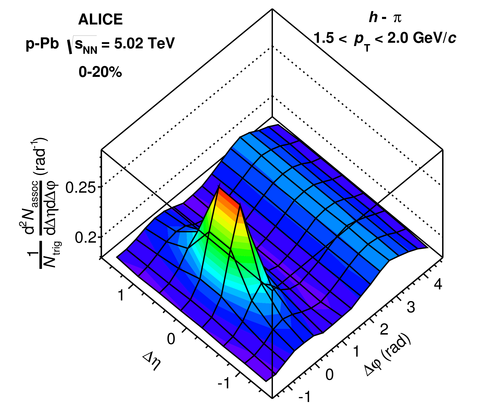
\includegraphics[width=1\textwidth]{main.png}}
			\caption{Экспериментальное распределение числа частиц по $\br{\Delta \eta, \Delta \phi}$  }
		\end{figure}
	\end{minipage}
\end{frame}

\begin{frame}[fragile]
    \frametitle{Цели}    
	\begin{minipage}[h]{0.45\linewidth}
		{\bf Глобальная цель: }
		Построить простую модель на основе струнной феноменологии для объяснения поведения $(\Dphi, \Dy)$ - корреляций. Найти аналитический вид зависимости $\rho(\Dphi, \Dy)$.
		\\
		{\bf Цель данной работы: }
		Построить модель объясняющую передний пик в  распределении $\rho(\Dphi, \Dy)$ и найти формулу для него.
	\end{minipage}
	\begin{minipage}[h]{0.53\linewidth}
		\begin{figure}
			\center{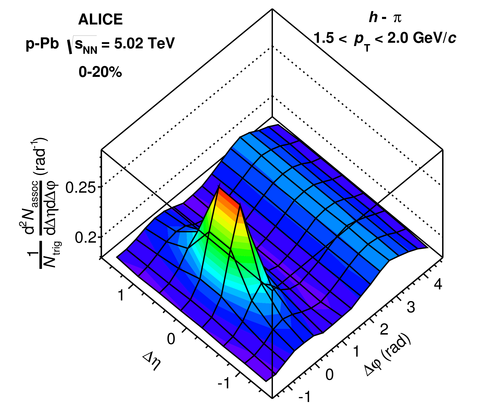
\includegraphics[width=1\textwidth]{main.png}}
			\caption{Экспериментальное распределение числа частиц по $\br{\Delta \eta, \Delta \phi}$  }
		\end{figure}
	\end{minipage}
\end{frame}

\begin{frame}[fragile]
    \frametitle{Формализация задачи}    
		\begin{minipage}[h]{0.49\linewidth}
			$\vec R, M$ - импульс и масса $\rho$-мезона, \\
			$\vec p_1, \vec p_2$ - импульсы $\pi$-мезонов, \\
			$m$ - масса $\pi$-мезонов
			\begin{gather*}
				\vec R = \vec p_1 + \vec p_2 \\
				\vec p_1, \vec p_2 \rightarrow \vec k, -\vec k
			\end{gather*}
		\end{minipage}
		\begin{minipage}[h]{0.49\linewidth}
			\begin{gather*}
				\begin{cases}
					tg\ \phi_1 = \frac{p_{1y}}{p_{1x}} = \frac{k_y}{R / 2 +  k_x \sqrt{1 + R^2 / M^2}} \\
					tg\ \phi_2 = \frac{p_{2y}}{p_{2x}} = -\frac{k_y}{R / 2 -  k_x \sqrt{1 + R^2 / M^2}} \\
					y_1 = \frac{1}{2} ln \frac{E_1 + p_{1z}}{E_1 - p_{1z}} = \frac{1}{2} ln \frac{E_1 + k_z}{E_1 - k_z} \\
					y_2 = \frac{1}{2} ln \frac{E_2 + p_{2z}}{E_2 - p_{2z}} = \frac{1}{2} ln \frac{E_2 - k_z}{E_2 + k_z} \\
				\end{cases}
			\end{gather*}
		\end{minipage}
		\begin{gather*}
			tg \Dphi = \frac{\pm R\sqrt{k^2 - k_x^2 - k_z^2}}{R^2 / 4 - k^2 - k_x^2 R^2 / M^2 + k_z^2} \\
			\Dy = \frac{1}{2} ln \frac{(R^2 + M^2) / 4 - \kxx R^2 / M^2 + \kzz +\kz \sqrt{R^2 + M^2}}{(R^2 + M^2) / 4 - \kxx R^2 / M^2 + \kzz -\kz \sqrt{R^2 + M^2}}
		\end{gather*}
\end{frame}

\begin{frame}[fragile]
    \frametitle{Распределение $\rho (\Dphi, \Dy)$}    
	\begin{gather*}
		\rho(\Dphi, \Dy) = \det{\Dphi, \Dy}{\kx,\kz} \rho(\kx, \kz) \propto \det{\kx,\kz}{\Dphi, \Dy} \frac{1}{\sqrt{k^2 - \kxx - \kzz}} \\
		\\
		\pa\ra\pb\ra\pc\ra\pd\ra\pe \\
		\\
		x = \kxx R^2 / M^2  + k^2 - \kzz - R^2 / 4 \\
		\y = \frac{k^2 + M^2/4 - x + \kz \sqrt{R^2 + M^2}}{k^2 + M^2/4 - x - \kz \sqrt{R^2 + M^2}} \\
		\f =  \frac{1}{x}\sqrt{(R^2 + M^2)k^2 - u^2 (k^2 + M^2 / 4 - x)^2 - M^2 x - M^2 R^2 / 4} \\
		\Dphi = arctg\f, \Dy = \frac{1}{2} ln \y \\
	\end{gather*}    
\end{frame}

\begin{frame}[fragile]
   \frametitle{Распределение $\rho (\Dphi, \Dy)$}    
	\begin{gather*}
		\rho(\Dphi, \Dy) = \det{\Dphi, \Dy}{\kx,\kz} \rho(\kx, \kz) \propto \det{\kx,\kz}{\Dphi, \Dy} \frac{1}{\sqrt{k^2 - \kxx - \kzz}} \\
		\\
		\pa\ra\pb\ra\pc\ra\pd\ra\pe \\
		\\
		\det{\pa}{\pe} = \det{\pa}{\pb}\det{\pb}{\pc}\det{\pc}{\pd}\det{\pd}{\pe} \\
		= \dff{\kx}{\pb}{x}{\kz} \cdot \dff{\kz}{\pc}{Y}{x} \cdot \dff{x}{\pd}{\f}{Y} \cdot \dff{\f}{\pe}{\Dphi}{\Dy} \cdot \dff{Y}{\pe}{\Dy}{\Dphi} \\
	\end{gather*}    
\end{frame}

\begin{frame}[fragile]
    \frametitle{Результат вычислений}    
	\begin{minipage}[h]{0.49\linewidth}
		\begin{figure}
			\center{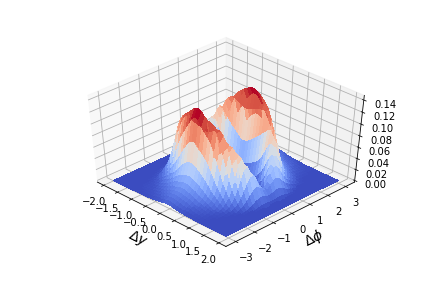
\includegraphics[width=1\textwidth]{R1.png}}
			\caption{Распределение числа частиц $\rho \br{\Dy, \Delta \phi}$ для $R = 1 GeV$}
		\end{figure}
	\end{minipage}
	\begin{minipage}[h]{0.49\linewidth}
		\begin{figure}
			\center{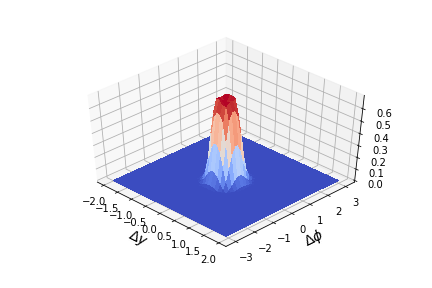
\includegraphics[width=1\textwidth]{R5.png}}
			\caption{Распределение числа частиц $\rho\br{\Dy, \Delta \phi}$ для $R = 5 GeV$}
		\end{figure}
	\end{minipage}
\end{frame}

\begin{frame}[fragile]
    \frametitle{Задний ридж}
	\begin{center}
		\begin{tikzpicture}
			\draw[very thick] (-3, 0) coordinate (Q0) circle (0.3);
			\draw[very thick] (-2, 0) coordinate (Q2) circle (0.3);
			\draw[thick] (Q0) +(90: .4) coordinate (A1) arc (90:270:0.4) coordinate (A3);
			\draw[thick] (Q2) +(90: .4) coordinate (A2) arc (90:-90:0.4) coordinate (A4);
			\draw[thick] (A1) -- (A2) (A3) -- (A4);

			\draw[very thick] (-1, 0) coordinate (Q1) circle (0.3);
			\draw[very thick] ( 0, 0) coordinate (Q2) circle (0.3);
			\draw[thick] (Q1) +(90: .4) coordinate (A1) arc (90:270:0.4) coordinate (A3);
			\draw[thick] (Q2) +(90: .4) coordinate (A2) arc (90:-90:0.4) coordinate (A4);
			\draw[thick] (A1) -- (A2) (A3) -- (A4);

			\draw[very thick] ( 1, 0) coordinate (Q1) circle (0.3);
			\draw[very thick] ( 2, 0) coordinate (Q2) circle (0.3);
			\draw[thick] (Q1) +(90: .4) coordinate (A1) arc (90:270:0.4) coordinate (A3);
			\draw[thick] (Q2) +(90: .4) coordinate (A2) arc (90:-90:0.4) coordinate (A4);
			\draw[thick] (A1) -- (A2) (A3) -- (A4);
			
			\draw[->] (Q0) +(-0.4, 0) -- +(-1,0);
			\draw[->] (Q2) +( 0.4, 0) -- +( 1,0);
		\end{tikzpicture}
	\end{center}
	\begin{minipage}[h]{0.50\linewidth}
		Разность быстрот между соседними фрагментами:
		$$ \Dy \approx \pm 1$$
		\\
		Распределение по $\Dphi$:
		\begin{gather*}
			\rho_{\Delta \phi} \br{\Delta \phi} = \qquad \qquad \qquad \qquad \\ 
			= \frac{3}{8 \pi} \frac{\sqrt{1 - \gamma^2} - \gamma \ arccos \gamma}{\br{1 - \gamma^2}^{3/2}},
		\end{gather*}
		$\quad \text{где} \ \gamma = \frac{cos \Delta \phi}{2}.$
	\end{minipage}
	\begin{minipage}[h]{0.49\linewidth}
			\begin{figure}
			\center{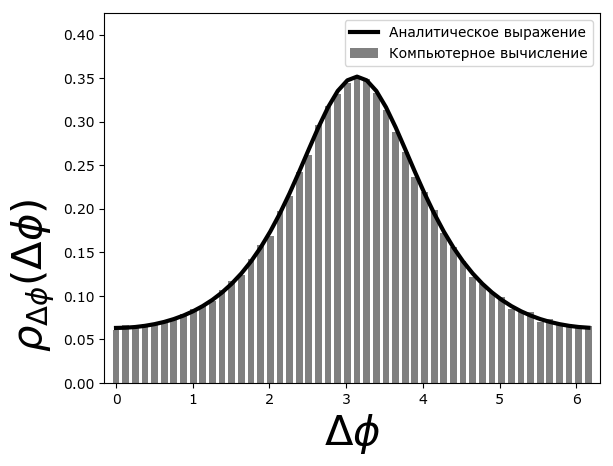
\includegraphics[width=1\textwidth]{gauss.png}}
			\caption{Распределение числа частиц $\rho_{\Delta \phi} \br{\Delta \phi}$ для сечения $ \Dy = \pm 1$}
		\end{figure}
	\end{minipage}
\end{frame}

\begin{frame}[fragile]
    \frametitle{Схема объединения распределений}  
	\begin{minipage}[h]{0.45\linewidth}
		\begin{figure}
			\center{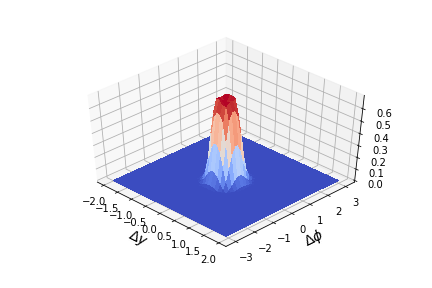
\includegraphics[width=1\textwidth]{R5.png}}
		\end{figure}
	\end{minipage}
	{\Large $+$}
	\begin{minipage}[h]{0.4\linewidth}
		\begin{figure}
			\center{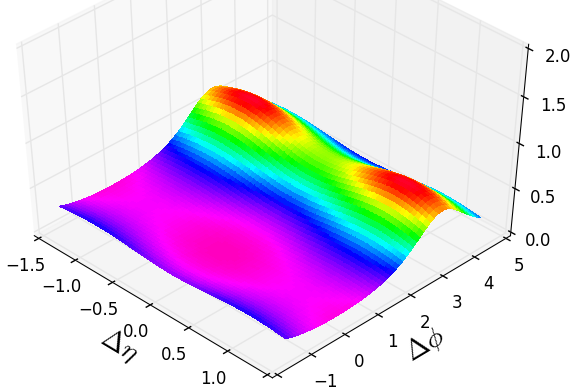
\includegraphics[width=1\textwidth]{must_be.png}}
		\end{figure}
	\end{minipage}
	\\
	\begin{center}
	{\Large$\approx$}
	\begin{minipage}[h]{0.4\linewidth}
		\begin{figure}
			\center{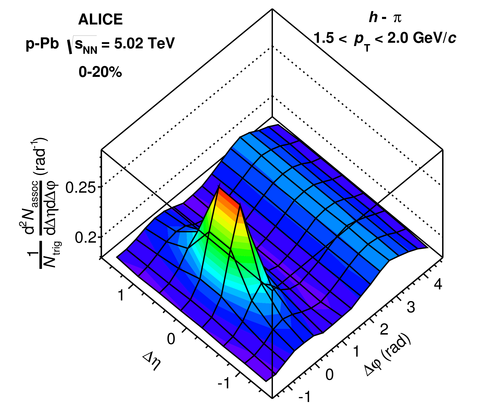
\includegraphics[width=1\textwidth]{main.png}}
		\end{figure}
	\end{minipage}
	\end{center}
\end{frame}

% \begin{frame}[fragile]
    % \frametitle{HBT}
% \end{frame}

\begin{frame}[fragile]
    \frametitle{Результаты}
	\begin{itemize}
		\item Была построена модель объясняющая образование переднего пика посредством влияния распада $\rho$-резонансов. Модель может использоваться как составная часть более сложных моделей.
		\item Для  $\rho (\Dy, \Dphi)$ удалось найти аналитическую формулу. Она может быть использованна для аппроксимации экспериментальных данных, нахождения параметров столкновения и их погрешностей.
	\end{itemize}
\end{frame}

\end{document}
